%
% filter.tex -- Paper zum Thema Optische Fouriertransformation <opt>
%
% (c) 2023 Marco Niederberger, Yanick Schoch; OST Ostschweizer Fachhochschule
%
% !TEX root = ../../buch.tex
% !TEX encoding = UTF-8
%
\section{Filter
\label{opt:section:filter}}
\rhead{Filterdesign}

Auch bei der optischen Fouriertransformation kann das Signal anschliessend in der Fourierebene bearbeitet werden.
Im optischen entspricht dies einer Blende.
Diese wird, wie in Abbildung \ref{opt:fig:4fAufbau} gezeigt, zwischen den beiden Linsen platziert.
Typische Filter in der Elektrotechnik sind Tiefpass, Hochpass, Bandpass und Bandsperre.
Deren Realisierung in der Optik ist in Abbildung \ref{opt:fig:filterarten} ersichtlich.

Im Nullpunkt der Filterebene sind die tiefen Frequenzen (DC-Anteil) und entlang der Achsen die höheren Frequenzen zu erkennen.
Somit entspricht eine lichtundurchlässige Fläche mit einem Loch in der Mitte einem Tiefpass und eine lichtundurchlässige Scheibe einem Hochpass.
Nach diesem Prinzip lassen sich auch die weiteren typischen Filter realisieren.

\subsection{Vergleich mit Filter 1. / 2. Ordnung}

\subsection{Cutoff Frequenz, Abfall nach $\omega_c$}

\subsection{Wo ist welche Frequenz $Hz <=> mm$ auf der Fourierebene}
Evt Formel in Abhängigkeit von der Wellenlänge, Distanz und Brennweite

\begin{figure}
    \centering
    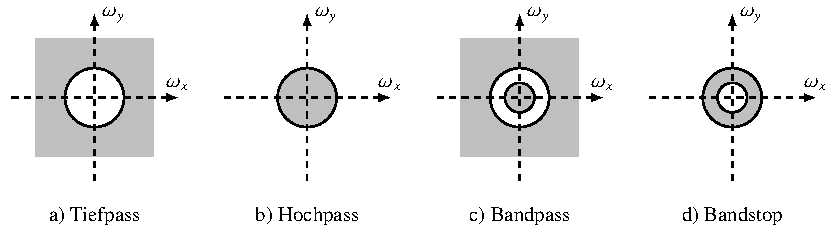
\includegraphics[width=\textwidth]{papers/opt/images/filterarten.pdf}

    \caption{Realisierung typischer Filter als optische Systeme;
        wobei grau lichtundurchlässig und weiss lichtdurchlässig bedeutet.}
    \label{opt:fig:filterarten}
\end{figure}
